
I diagrammi di comunicazione mostrano il comportamento dinamico di uno use-case, evidenziando l'interazione fra i componenti del sistema per il raggiungimento di un risultato.

In figura~\ref{fig:communication:obp} è illustrata la sequenza di azioni necessarie per l'invio di un'operazione al back-end della banca tramite l'interfaccia OBP.

\begin{figure*}[h]
    \centering
    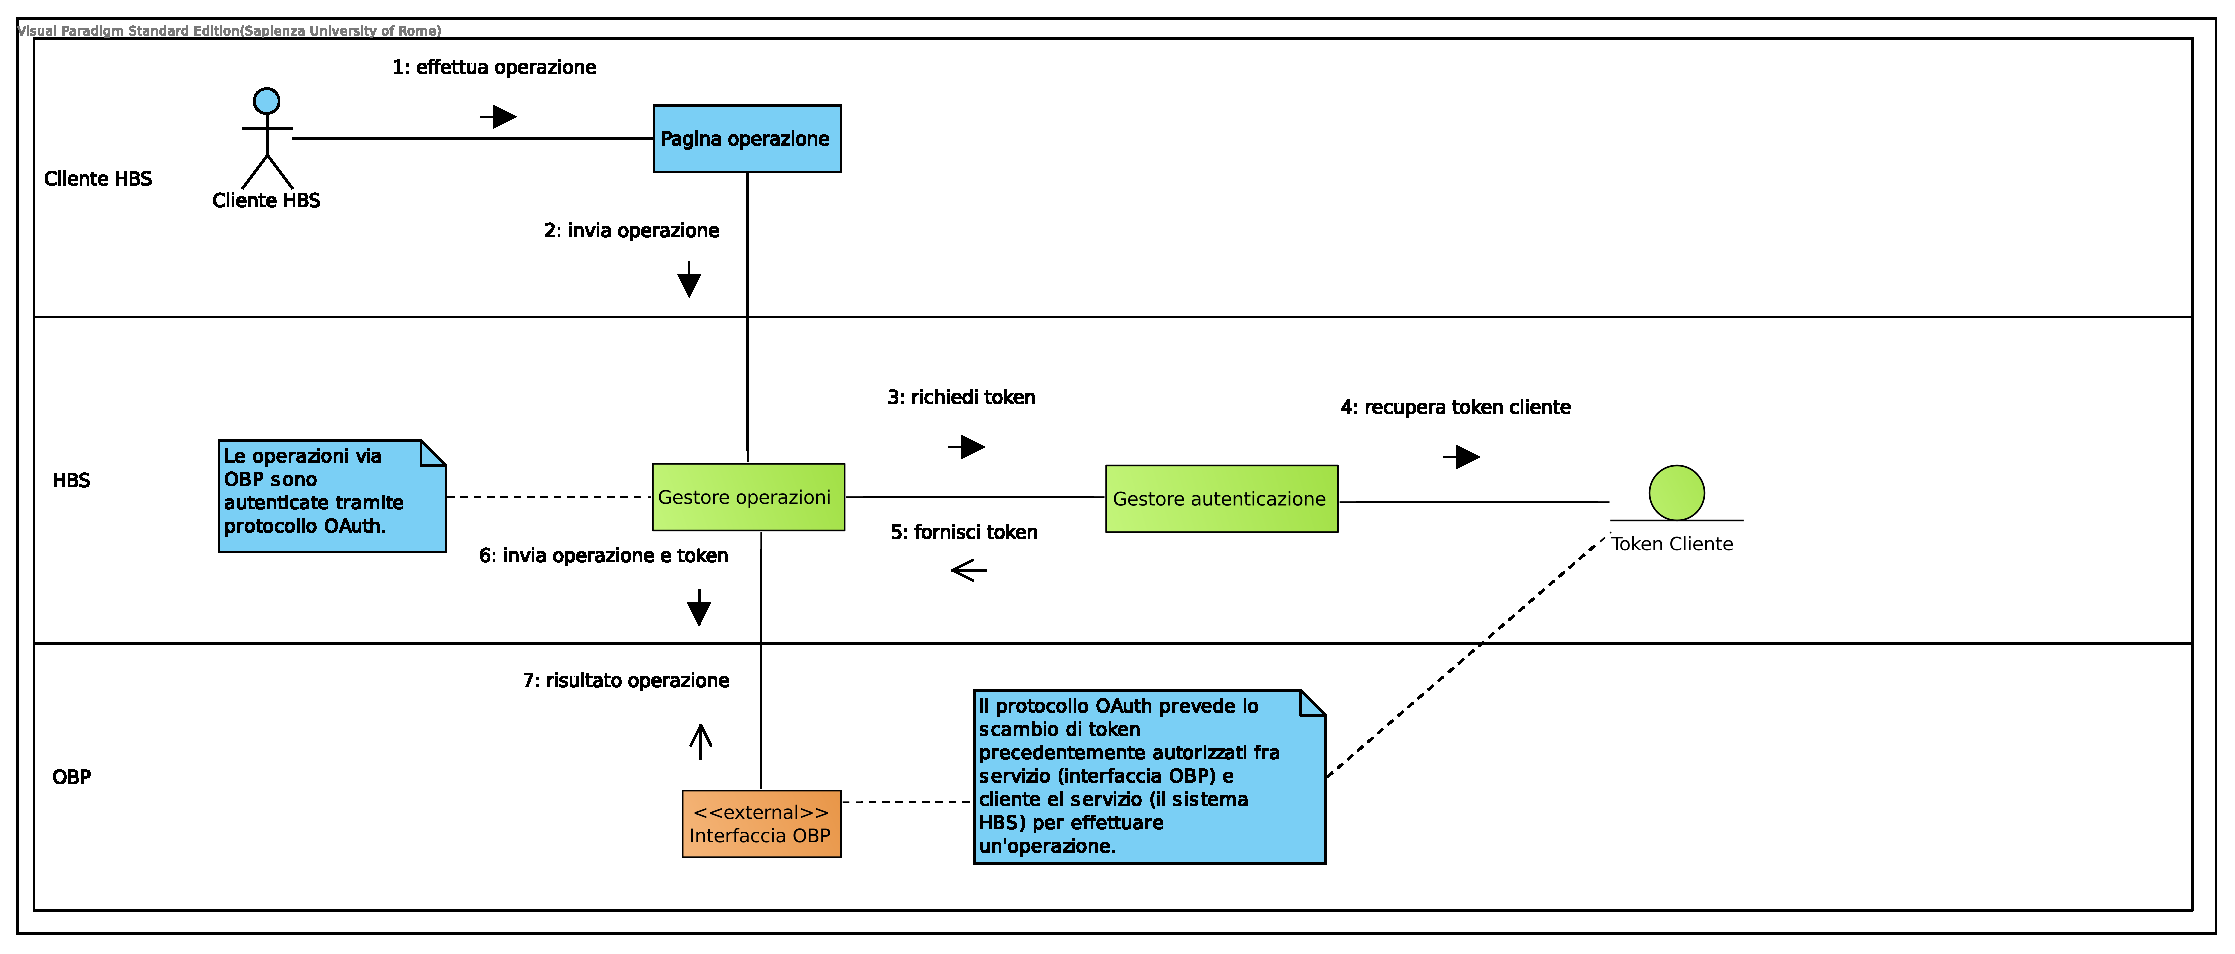
\includegraphics[width=\textheight, angle=90]{Images/Comunicazione_OBP.eps}
    \caption{Diagramma di comunicazione per l'esecuzione di operazioni.}
    \label{fig:communication:obp}
\end{figure*}


